% User guide: http://mirrors.ctan.org/macros/latex/contrib/bookcover/bookcover.pdf
% A4 size 210 x 297 mm
% shenweis685@gmail.com
% 做封面寬(210+210+書背厚度 17.8mm)X 高29.7公分; 上下留白各2-3公分
\documentclass[
    coverwidth=210mm, %213mm, %150mm,
    coverheight=297mm, %303mm, %200mm,高29.7公分
    spinewidth=17.8mm, % 289 pages, 米色道林紙 100g
%    flapwidth=6cm,
%    wrapwidth=5mm,
%    trimmed % Show only trimmed part!
%    bleedwidth=3mm,
    12pt,
    trimmed=false %true
    ]{bookcover}

%\bookcovertrimmedpart{front} % Trimmed part is the front cover
%\bookcovertrimmedpart{back} % Trimmed part is the back cover
%\bookcovertrimmedpart{spine} % Trimmed part is the spine

\newbookcovercomponenttype{center rotate}{
    \vfill
    \centering
    \rotatebox[origin=c]{-90}{#1}
    \vfill}

\usepackage[outline]{contour}% It doesn't work with xelatex and lualatex
\contourlength{1pt}
\usepackage[english]{babel}
\usepackage{kantlipsum,microtype}

% Chinese
\usepackage{xeCJK} % for Chinese, compiling by XeLaTex

\usepackage{fontspec} %設定字體
% Fandol font (the default)  not shown "內"
\setCJKmainfont{AR PL UMing TW MBE} % AR PL UMing TW MBE or "UKai" https://www.overleaf.com/learn/latex/Questions/Which_OTF_or_TTF_fonts_are_supported_via_fontspec%3F#Chinese
%BiauKai} %標楷體 from macOS %設定中文為系統上的字型,而英文不去更動,使用原TeX字型
%\setCJKmainfont[Vertical=RotatedGlyphs]{AR PL UMing TW MBE}

\begin{document}

\begin{bookcover}

% Remark
%\begin{bookcoverelement}{center}{above front}
%    \textcolor{blue}{A dust jacket example}
%\end{bookcoverelement}

% Background color on the whole cover
\begin{bookcoverelement}{color}{bg whole}
    white
\end{bookcoverelement}

% Background picture on the whole cover without flaps
\begin{bookcoverelement}{picture}{bg whole without flaps}
    %./figures/bookcover-bg.jpg
\end{bookcoverelement}

% Transparent areas on the back cover
%\begin{bookcoverelement}{tikz}{bg back and wrap}
%    \fill[opacity=0.3,black!50] 
%    (0,0) rectangle (25mm,\partheight) 
%    (part.north east) rectangle ([xshift=-5cm]part.south east);
%\end{bookcoverelement}

% Transparent areas on the front cover
%\begin{bookcoverelement}{tikz}{bg front and wrap}
%    \fill[opacity=0.3,black!50] 
%    (0,0) rectangle (50mm,\partheight) 
%    (part.north east) rectangle ([xshift=-25mm]part.south east);
%\end{bookcoverelement}

% Picture on the front cover behind the title
\begin{bookcoverelement}{center}{front}
    %
\includegraphics{watermarkTMU.jpg}
    %{./figures/bookcover-cards.pdf}
\end{bookcoverelement}

% Author and title on the front cover
\begin{bookcoverelement}{normal}{front}[,3cm,,3cm]
    \centering % yellow!60!
    \color{black}\sffamily\bfseries
    \resizebox{!}{7mm}{
        臺北醫學大學}\\[3mm]
    \resizebox{!}{7mm}{%\contour{black}{}
        轉譯醫學博士學位學程
    }\\[3mm]
    \resizebox{!}{7mm}{
        博士論文
    %The Ph.D. Program for 
    }\\[3mm]
    \resizebox{!}{5mm}{
    Taipei Medical University}\\[3mm]
    \resizebox{!}{5mm}{%\contour{black}{}
    The Ph.D. Program
    }\\[3mm]
    \resizebox{!}{5mm}{%\contour{black}{}
    for Translational Medicine
    }\\[4mm]
    \resizebox{!}{5mm}{
    Doctoral Dissertation
    %The Ph.D. Program for 
    }\\[10mm]
    \parbox{160mm}{ %linewidth=
    {\bfseries\huge
    以全基因轉錄組和蛋白質體分析來鑑定\\[2mm]
    驗證頭頸部鱗狀上皮細胞癌的生物標記\\[4mm]
    Global Transcriptomics and Proteomics Analyses for Biomarker Identification and Validation in Head and Neck Squamous Cell Carcinoma}}\\[7mm]
    \resizebox{!}{7mm}{
    研究生:祁力行撰}\\[2mm]
    \resizebox{!}{4mm}{
    Graduate Student: Li-Hsing Chi}\\[4mm]
    \resizebox{!}{7mm}{
    指導教授:李友專教授}\\[2mm]
    \resizebox{!}{4mm}{
    Advisor: 
    Yu-Chuan (Jack) Li, M.D., Ph.D.}\\[4mm]
    \resizebox{!}{7mm}{
    指導教授: 蕭宏昇博士}\\[2mm]
    \resizebox{!}{4mm}{
    Advisor:
    Michael Hsiao, D.V.M., Ph.D.}\\[4mm]
    \resizebox{!}{7mm}{
    共同指導教授:吳駿翃副教授}\\[2mm]
    \resizebox{!}{4mm}{
    Co-Advisor: 
    Alexander Jun-Hong Wu, Ph.D.}\\[7mm]
    \resizebox{!}{6mm}{
    \small 中華民國一百一十一年元月}\\[2mm]
    \resizebox{!}{4mm}{
    \small 2022.01}%\\[26mm]

%\author{Li-Hsing Chi}
%\degreemonth{January}
%\degreeyear{2022} 
%\dissertation
%\doctorphilosophy
%%% \normalsize
%\noindent {\bf{Primary Advisors:}} 
%Yu-Chuan (Jack) Li,
%\indent\indent\indent\indent\indent\indent
%Michael Hsiao\\
%{\bf{Secondary Advisor:}} 
%Alexander TH Wu\\
\end{bookcoverelement}



% Title on the spine
\begin{bookcoverelement}{normal}{spine}[4.5mm,30mm,0mm,21mm]
% center rotate
    %\color{yellow!60!black}
    %\contour{black}
\rotatebox[origin=c]{0}{\large\sffamily\bfseries
% or rotate -90
\parbox{30mm}{ %55
轉臺\\
譯北\\
醫醫\\
學學\\
博大\\
士學\\
學\\
位\\
學\\
程\\[3mm]
%\parbox{40mm}{
{ \hspace{10mm} 
論博\\
文士
}\\[3mm]
%\parbox{90mm}{
驗以\\
證全\\
頭基\\
頸因\\
部轉\\
鱗錄\\
狀組\\
上和\\
皮蛋\\
細白\\
胞質\\
癌體\\
的分\\
生析\\
物來\\
標鑑\\
記定\\[3mm]
%\parbox{40mm}{
{ \hspace{25mm}
祁\\
力\\
行
}\\[3mm]
%\parbox{70mm}{
一中\\
十華\\
一民\\
年國\\
元一\\
月百\\
\
} % end of parabox
}
%\parbox{30mm}{\indent 祁}
%    {Li-Hsing Chi -- Bioinformatic Study of HNSCC -- 2022.01}
\end{bookcoverelement}






\end{bookcover}

\end{document}
%%
% Text on the back cover
\begin{bookcoverelement}{normal}{back}[2cm,2cm,2cm,2cm]
    \color{gray}%\kant[1]
    %\begin{keywords}
{\large KEYWORDS:\\}
Head and Neck Squamous Cell Carcinoma (HNSCC),
Biomedical Informatics,
Forensic Medicine,
TCGA,
RNA-sequencing,
Survival Analysis,
Optimal Cutoff, Sliding-window Cutoff,
Kaplan--Meier Survival Analysis, Cox Proportional Hazard Model,
Biomarker,
%Tumor Type-agnostic Therapy,
%Immuno-Oncology,
%Targeted Therapy,
Systemic Therapy,
Surgical Margin,
Tobacco, Betel nut,
Rstudio, R, C++, Deep Learning,
Holistic Cancer Care,
%Therapeutic Relationship,
Mindfulness Meditation,
Thymosin Beta-4 X-linked (TMSB4X), %\capitalisewords{}
Calcium/calmodulin Dependent Protein Kinase II Inhibitor 1 (CAMK2N1),
Calmodulin like 5 (CALML5),
Fc Fragment of IgG Binding Protein (FCGBP)

\end{bookcoverelement}

% Text and picture on the front flap
%\begin{bookcoverelement}{normal}{front flap}[1cm,1cm,1cm,2cm]
%    \color{white}\kant[2]
%    \vfill
%    {\centering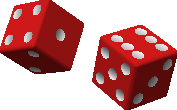
\includegraphics{./figures/bookcover-dice.pdf}\par}
%\end{bookcoverelement}

% Text on the back flap
%\begin{bookcoverelement}{normal}{back flap}[1cm,2cm,1cm,2cm]
%    \color{white}\kant[3]
%\end{bookcoverelement}
